\documentclass[12pt,a4paper]{article}

% ─── Page Layout ───────────────────────────────────────────────────────────────
\usepackage[a4paper, margin=0.8in, headheight=14pt]{geometry}

% ─── Fonts (XeLaTeX) ───────────────────────────────────────────────────────────
\usepackage{fontspec}
\usepackage{unicode-math}
\setmainfont{TeX Gyre Pagella}
\setmonofont[Scale=0.88]{TeX Gyre Cursor}
\setmathfont{Latin Modern Math}

% ─── Packages ──────────────────────────────────────────────────────────────────
\usepackage{xcolor}
\usepackage{colortbl}
\usepackage{titlesec}
\usepackage{enumitem}
\usepackage{tabularx}
\usepackage{booktabs}
\usepackage{array}
\usepackage{amsmath}
\usepackage{tikz}
\usetikzlibrary{shapes.geometric, arrows.meta, positioning, calc, fit, decorations.pathreplacing, patterns, backgrounds}
\usepackage{tcolorbox}
\tcbuselibrary{skins, breakable}
\usepackage{hyperref}
\usepackage{fancyhdr}
\usepackage{graphicx}
\usepackage{microtype}
\hyphenpenalty=10000
\exhyphenpenalty=10000
\sloppy
\usepackage{caption}
\usepackage{setspace}
\usepackage{multirow}
\usepackage{tocloft}

% ─── Q&A helper ────────────────────────────────────────────────────────────────
\newcommand{\Q}[1]{\textbf{#1}\par\noindent\ignorespaces}

% ─── Colour Palette ────────────────────────────────────────────────────────────
\definecolor{myred}{RGB}{196,30,58}
\definecolor{mydark}{RGB}{30,30,50}
\definecolor{mygreen}{RGB}{14,120,80}
\definecolor{myteal}{RGB}{0,130,140}
\definecolor{myamber}{RGB}{180,100,0}
\definecolor{mypurple}{RGB}{100,30,160}
\definecolor{mygray}{RGB}{246,247,249}
\definecolor{mgframe}{RGB}{180,185,200}
\definecolor{watermark}{RGB}{145,150,170}
\definecolor{hdrred}{RGB}{250,232,235}
\definecolor{hdrgreen}{RGB}{220,244,233}
\definecolor{hdrteal}{RGB}{220,242,244}
\definecolor{hdramber}{RGB}{253,242,215}
\definecolor{hdrpurple}{RGB}{238,228,255}
\definecolor{hdrgray}{RGB}{238,240,245}
\definecolor{rowalt}{RGB}{250,251,253}

% ─── Section Formatting ────────────────────────────────────────────────────────
\titleformat{\section}{\large\bfseries\color{myred}}{\thesection.}{0.5em}{}[\vspace{1pt}{\color{myred}\rule{\linewidth}{0.8pt}}]
\titleformat{\subsection}{\normalsize\bfseries\color{myteal}}{\thesubsection}{0.5em}{}
\titlespacing*{\section}{0pt}{18pt}{7pt}
\titlespacing*{\subsection}{0pt}{11pt}{4pt}

% ─── Paragraph ─────────────────────────────────────────────────────────────────
\setlength{\parindent}{0pt}
\setlength{\parskip}{4pt}

% ─── TOC Styling ───────────────────────────────────────────────────────────────
\renewcommand{\cfttoctitlefont}{\large\bfseries\color{myred}}
\renewcommand{\cftaftertoctitle}{\par\noindent{\color{myred}\rule{\linewidth}{0.8pt}}}
\setlength{\cftbeforetoctitleskip}{0pt}
\setlength{\cftaftertoctitleskip}{6pt}
\renewcommand{\cftsecfont}{\normalsize\bfseries\color{mydark}}
\renewcommand{\cftsecpagefont}{\normalsize\bfseries\color{mydark}}
\renewcommand{\cftsecleader}{\cftdotfill{\cftdotsep}}
\setlength{\cftbeforesecskip}{7pt}
\renewcommand{\cftsubsecfont}{\small\color{mydark}}
\renewcommand{\cftsubsecpagefont}{\small\color{mydark}}
\setlength{\cftbeforesubsecskip}{3pt}
\setlength{\cftsubsecindent}{1.4em}

% ─── Table helpers ─────────────────────────────────────────────────────────────
\renewcommand{\arraystretch}{1.45}
\setlength{\tabcolsep}{6pt}
\arrayrulecolor{mydark}
\newcolumntype{B}[1]{>{\small\bfseries\raggedright\arraybackslash}m{#1}}
\newcolumntype{Y}{>{\small\raggedright\arraybackslash}X}
\renewcommand{\tabularxcolumn}[1]{m{#1}}

% ─── Header / Footer ───────────────────────────────────────────────────────────
\pagestyle{fancy}
\fancyhf{}
\fancyhead[L]{\small\color{myred}\textbf{OE-EC803B}\;\color{mydark}--- Big Data Analysis}
\fancyhead[R]{\small\color{myteal}\textbf{Module 1 Notes}}
\fancyfoot[C]{\small\color{mydark}\thepage}
\fancyfoot[R]{\small\color{watermark}\textit{\copyright\ Biraj Sarkar}}
\renewcommand{\headrulewidth}{0.5pt}
\renewcommand{\footrulewidth}{0.3pt}

% ─── Hyperref ──────────────────────────────────────────────────────────────────
\hypersetup{colorlinks=true, linkcolor=myteal, urlcolor=myteal,
  pdfauthor={Biraj Sarkar}, pdftitle={OE-EC803B --- Module 1 Notes}}

% ─── tcolorbox styles ──────────────────────────────────────────────────────────
\tcbset{
  tikzbox/.style={colback=mygray, colframe=mgframe, boxrule=0.6pt, arc=4pt,
    left=8pt, right=8pt, top=6pt, bottom=6pt,
    colbacktitle=mgframe, coltitle=mydark, fonttitle=\small\bfseries, unbreakable},
  defbox/.style={colback=hdrgreen, colframe=mygreen, boxrule=0.8pt, arc=4pt,
    left=9pt, right=9pt, top=6pt, bottom=6pt,
    colbacktitle=mygreen, coltitle=white, fonttitle=\small\bfseries},
  formulabox/.style={colback=hdrteal, colframe=myteal, boxrule=0.8pt, arc=4pt,
    left=9pt, right=9pt, top=7pt, bottom=7pt,
    colbacktitle=myteal, coltitle=white, fonttitle=\small\bfseries},
  examplebox/.style={colback=hdramber, colframe=myamber, boxrule=0.8pt, arc=4pt,
    left=9pt, right=9pt, top=6pt, bottom=6pt,
    colbacktitle=myamber, coltitle=white, fonttitle=\small\bfseries},
  masonbox/.style={colback=hdrpurple, colframe=mypurple, boxrule=0.8pt, arc=4pt,
    left=9pt, right=9pt, top=6pt, bottom=6pt,
    colbacktitle=mypurple, coltitle=white, fonttitle=\small\bfseries},
  exambox/.style={colback=hdrpurple, colframe=mypurple, boxrule=1pt, arc=5pt,
    left=10pt, right=10pt, top=8pt, bottom=8pt,
    colbacktitle=mypurple, coltitle=white, fonttitle=\bfseries,
    breakable, title after break={\textbf{Frequently Asked / Viva Questions (contd.)}}}
}
\tcbset{breakable}

% ─── TikZ styles ───────────────────────────────────────────────────────────────
\tikzset{
  block/.style={rectangle, draw=myteal, fill=hdrteal,
    text width=2.4cm, align=center, minimum height=0.95cm,
    font=\small, rounded corners=3pt, line width=0.7pt},
  redblock/.style={rectangle, draw=myred, fill=hdrred,
    text width=2.4cm, align=center, minimum height=0.95cm,
    font=\small, rounded corners=3pt, line width=0.7pt},
  arrow/.style={-Stealth, thick, color=mydark},
  line/.style={thick, color=mydark}
}

\begin{document}

% ═══════════════════════════════════════════════════════════════════════════════
% TITLE BLOCK
% ═══════════════════════════════════════════════════════════════════════════════
\begin{center}
  \hfill \textit{Exam-Ready Short Notes} \\
  \vspace{6pt}
  {\LARGE\bfseries\color{myred} OE-EC803B --- Big Data Analysis}\\[5pt]
  {\normalsize\color{mydark} Semester VIII \quad$\bullet$\quad 3L:0T:0P \quad$\bullet$\quad 3 Credits}\\[3pt]
  {\normalsize\color{myteal}\textbf{Module 1: Introduction to Big Data \& Hadoop Ecosystem}}\\[3pt]
  {\small\color{mydark} CGEC \;$|$\; B.Tech ECE (2023--27) \;$|$\; \textit{Biraj Sarkar}}
\end{center}
\vspace{2pt}
\noindent{\color{myred}\rule{\linewidth}{1.5pt}}
\vspace{2pt}

\hypersetup{linkcolor=mydark}
\tableofcontents
\hypersetup{linkcolor=myteal}
\newpage

% ===============================================================================
\section{Types of Digital Data}
% ===============================================================================

Digital data represents any information stored, processed, or transmitted electronically. In modern computer systems, digital data is classified into three categories based on its structural characteristics:

\begin{tcolorbox}[defbox, title={Classification of Digital Data}]
  \textbf{Digital Data} is categorized into three types:
  \begin{enumerate}[leftmargin=*, noitemsep]
    \item \textbf{Structured Data:} Highly organized data conforming to a rigid pre-defined schema (e.g., relational databases).
    \item \textbf{Semi-Structured Data:} Data containing internal identifiers, tags, or markers (no rigid schema, but self-describing; e.g., JSON, XML).
    \item \textbf{Unstructured Data:} Data lacking any predefined structure or model (e.g., videos, PDF documents, raw text).
  \end{enumerate}
\end{tcolorbox}

\subsection{Detailed Characteristics}
\begin{itemize}[leftmargin=*, itemsep=4pt]
  \item \textbf{Structured Data:}
    Stored in tables with rows and columns. Uses Structured Query Language (SQL) for retrieval. It has fixed fields and schemas.
    \textit{Examples:} Relational Databases (RDBMS), CSV files, spreadsheets.
  \item \textbf{Semi-Structured Data:}
    Does not conform to the formal structure of databases but contains tags or markers to separate data elements and enforce hierarchies.
    \textit{Examples:} XML documents, JSON strings, HTML files, NoSQL Key-Value records.
  \item \textbf{Unstructured Data:}
    Represents the majority of real-world data (estimated at 80--90\% of all enterprise data). It is difficult to store in standard tabular formats.
    \textit{Examples:} MP3 files, MP4 videos, JPEG images, raw logs, emails, PDF manuals.
  \end{itemize}

\par\vspace{6pt}\noindent
{\renewcommand{\arraystretch}{1.4}%
\begin{tabularx}{\linewidth}{|B{2.8cm}|Y|Y|Y|}
\hline
\textbf{Parameter} & \textbf{Structured Data} & \textbf{Semi-Structured Data} & \textbf{Unstructured Data} \\
\hline
Format & Tabular (Rows/Columns) & Tags/Key-value pairs & No specific structure \\
\hline
Schema & Schema-on-write (rigid) & Schema-on-read (flexible) & No schema applied \\
\hline
Storage & RDBMS (SQL Server, MySQL) & NoSQL databases, XML files & NoSQL databases, Data Lakes \\
\hline
Flexibility & Very low & Moderate & High \\
\hline
Scale & Hard to scale horizontally & Scalable horizontally & Highly scalable \\
\hline
Querying & Structured SQL queries & XQuery, JSON Path & Search indices, NLP, ML \\
\hline
\end{tabularx}}

% ===============================================================================
\section{Introduction to Big Data}
% ===============================================================================

\begin{tcolorbox}[defbox, title={Big Data}]
  \textbf{Big Data} refers to datasets whose size (volume), complexity (variety), and rate of growth (velocity) are so large that traditional data processing application software (such as relational database management systems) are inadequate to capture, store, manage, and process them within a tolerable elapsed time.
\end{tcolorbox}

\subsection{The 5Vs of Big Data}
The core dimensions defining Big Data are historically known as the \textbf{3Vs} (Volume, Velocity, Variety), which have been expanded to the \textbf{5Vs} to reflect reliability and business value:

\begin{enumerate}[leftmargin=*, itemsep=3pt]
  \item \textbf{Volume:} The sheer scale of data generated. Measured in Terabytes (TB), Petabytes (PB), or Exabytes (EB).
  \item \textbf{Velocity:} The speed at which new data is generated, transmitted, and processed in real-time (e.g., social media feeds, sensor streams).
  \item \textbf{Variety:} The structural diversity of data types (structured, semi-structured, and unstructured data coming from various sources).
  \item \textbf{Veracity:} The trustworthiness, quality, and accuracy of the incoming data (noise reduction, handling missing values).
  \item \textbf{Value:} The actionable business insights extracted from the data, turning raw bits into commercial or operational intelligence.
\end{enumerate}

\begin{tcolorbox}[tikzbox, title={The 5Vs of Big Data}]
\centering
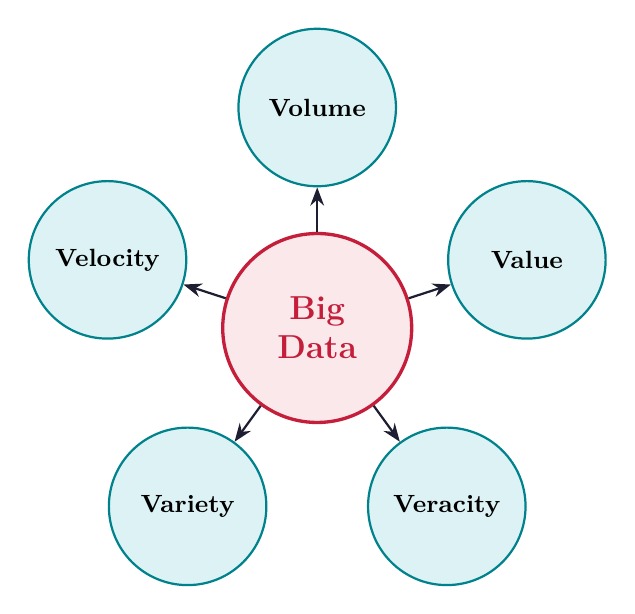
\begin{tikzpicture}[node distance=1.2cm,
  vnode/.style={circle, draw=myteal, fill=hdrteal, minimum size=2.0cm, align=center, font=\small\bfseries, line width=0.8pt},
  centerbox/.style={circle, draw=myred, fill=hdrred, minimum size=2.4cm, align=center, font=\large\bfseries\color{myred}, line width=1.2pt},
  carrow/.style={-Stealth, thick, color=mydark}]

  % Center node
  \node[centerbox] (bd) at (0,0) {Big\\Data};

  % Satellite nodes
  \node[vnode] (vol) at (90:2.8cm) {Volume};
  \node[vnode] (vel) at (162:2.8cm) {Velocity};
  \node[vnode] (var) at (234:2.8cm) {Variety};
  \node[vnode] (ver) at (306:2.8cm) {Veracity};
  \node[vnode] (val) at (18:2.8cm) {Value};

  % Connections
  \draw[carrow] (bd) -- (vol);
  \draw[carrow] (bd) -- (vel);
  \draw[carrow] (bd) -- (var);
  \draw[carrow] (bd) -- (ver);
  \draw[carrow] (bd) -- (val);

\end{tikzpicture}
\end{tcolorbox}

\subsection{Challenges of Traditional Database Systems (RDBMS)}
Traditional RDBMS architectures fail to handle Big Data due to several fundamental limits:
\begin{itemize}[leftmargin=*, itemsep=3pt]
  \item \textbf{Vertical Scaling (Scale-up) limits:} RDBMS scale by adding CPU, RAM, or storage to a single server. This has physical and cost limits. Big Data requires horizontal scaling (scaling out by adding cheap commodity nodes).
  \item \textbf{Rigid Schema Requirements:} RDBMS requires schema definitions before writing data. This prevents storing unstructured data or dynamic fields.
  \item \textbf{ACID Properties Overhead:} Locking rows/tables to maintain strict Consistency and Isolation creates severe latency spikes at high transaction speeds.
\end{itemize}

% ===============================================================================
\section{Big Data Analytics}
% ===============================================================================

\begin{tcolorbox}[defbox, title={Big Data Analytics}]
  \textbf{Big Data Analytics} is the process of examining large and varied datasets to uncover hidden patterns, unknown correlations, market trends, customer preferences, and other useful information to make informed business decisions.
\end{tcolorbox}

\subsection{Types of Big Data Analytics}
Analytics tasks are classified into four distinct stages based on complexity and value:

\begin{enumerate}[leftmargin=*, itemsep=3pt]
  \item \textbf{Descriptive Analytics (What happened?):} Summarizes historical data to identify trends and patterns (e.g., standard reports, dashboards).
  \item \textbf{Diagnostic Analytics (Why did it happen?):} Drill-down queries to identify the root cause of historical trends (e.g., analyzing customer churn).
  \item \textbf{Predictive Analytics (What is likely to happen?):} Uses statistical models, forecasting algorithms, and machine learning to estimate future outcomes.
  \item \textbf{Prescriptive Analytics (What should we do?):} Recommends action pathways based on simulations and optimization algorithms to capitalize on predictions.
\end{enumerate}

% ===============================================================================
\section{History and Architecture of Apache Hadoop}
% ===============================================================================

\subsection{History of Hadoop}
Hadoop was created by Doug Cutting and Mike Cafarella in 2005. It originated from work on Nutch, an open-source web crawler project.
\begin{itemize}[leftmargin=*, itemsep=3pt]
  \item It was inspired by Google's white papers on GFS (Google File System) published in 2003 and MapReduce framework published in 2004.
  \item Doug Cutting joined Yahoo! in 2006, and Yahoo! spun off Hadoop as an independent open-source project. In 2008, Apache Hadoop became a top-level project.
  \item Named after Doug Cutting's son's toy yellow elephant.
\end{itemize}

\subsection{Core Components of Apache Hadoop}
Hadoop provides a distributed software framework designed to run on clusters of commodity hardware.

\begin{tcolorbox}[formulabox, title={Core Hadoop Modules}]
  Hadoop's primary runtime architecture contains three core modules:
  \begin{enumerate}[leftmargin=*, noitemsep]
    \item \textbf{HDFS (Hadoop Distributed File System):} The distributed storage layer that splits files into blocks and distributes them across cluster nodes.
    \item \textbf{MapReduce:} The software programming framework for writing applications that process massive amounts of structured and unstructured data in parallel.
    \item \textbf{YARN (Yet Another Resource Negotiator):} The cluster resource management layer that schedules jobs and allocates CPU/RAM resources across the cluster.
  \end{enumerate}
\end{tcolorbox}

\subsection{Unix Tools vs. Hadoop}
Small datasets are processed locally using Unix utilities, whereas large datasets require distributed execution on Hadoop.

\par\vspace{6pt}\noindent
{\renewcommand{\arraystretch}{1.4}%
\begin{tabularx}{\linewidth}{|B{3.2cm}|Y|Y|}
\hline
\textbf{Parameter} & \textbf{Unix Utilities (grep, awk, sed)} & \textbf{Apache Hadoop} \\
\hline
Execution Location & Single local machine & Distributed cluster (scale-out) \\
\hline
Data Volume Limit & Limited by local RAM and disk size & Petabytes (scales linearly with nodes) \\
\hline
Processing Paradigm & Sequential processing (single-threaded pipes) & Parallel, distributed execution (MapReduce) \\
\hline
Fault Tolerance & None (if the shell script crashes, run aborts) & High (data blocks replicated; jobs rerun automatically) \\
\hline
Data Locality & Reads data to CPU over system bus & Pushes computation code directly to storage nodes \\
\hline
\end{tabularx}}

% ===============================================================================
\section{Hadoop Streaming}
% ===============================================================================

\begin{tcolorbox}[defbox, title={Hadoop Streaming}]
  \textbf{Hadoop Streaming} is a utility that comes bundled with the Hadoop distribution that allows users to create and run MapReduce jobs with any executable or script as the mapper and/or the reducer (e.g., Python, Perl, Bash) by exchanging data via standard input (`stdin`) and standard output (`stdout`).
\end{tcolorbox}

\subsection{Mechanism and Data Flow}
\begin{enumerate}[leftmargin=*, itemsep=3pt]
  \item The Java MapReduce program spawns the mapper as a separate process and pipes HDFS input data line-by-line to the mapper process's `stdin`.
  \item The mapper program reads lines from `stdin`, processes the data, and writes tab-separated key-value pairs to its `stdout`.
  \item The streaming utility intercepts `stdout` and handles sorting, partitioning, and shuffling to group keys together.
  \item The streaming utility spawns the reducer process and pipes the grouped key-value data to its `stdin`.
  \item The reducer reads from `stdin`, aggregates values, and writes output key-value lines to `stdout`, which are captured and stored in HDFS.
\end{enumerate}

\begin{tcolorbox}[examplebox, title={Example: Python Mapper Script for Streaming}]
\begin{spacing}{0.95}
\begin{verbatim}
import sys
# Mapper: Reads lines from stdin, splits into words, outputs key-value
for line in sys.stdin:
    words = line.strip().split()
    for word in words:
        # Output: word (key) <TAB> 1 (value)
        print(f"{word}\t1")
\end{verbatim}
\end{spacing}
\end{tcolorbox}

% ===============================================================================
\section{Hadoop Ecosystem}
% ===============================================================================

The Hadoop framework is surrounded by a set of specialized helper tools that together form the \textbf{Hadoop Ecosystem}:

\begin{tcolorbox}[tikzbox, title={Apache Hadoop Ecosystem Architecture}]
\centering
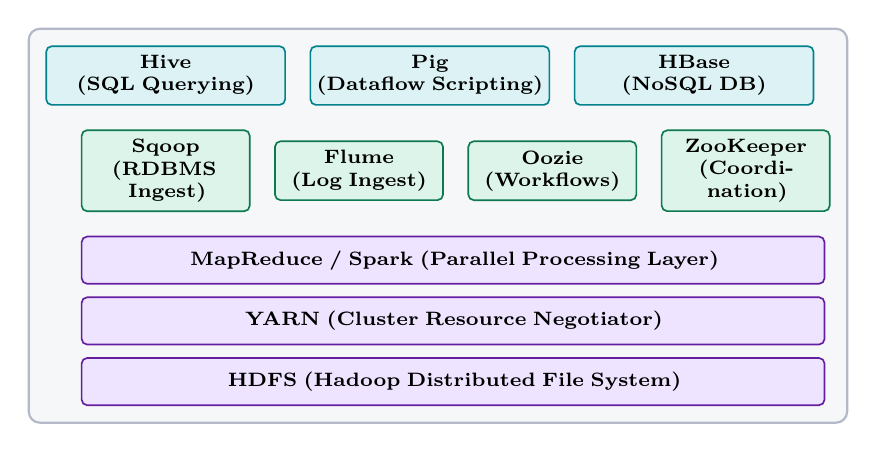
\begin{tikzpicture}[node distance=0.15cm and 0.2cm,
  sblock/.style={rectangle, draw=myteal, fill=hdrteal, text width=2.8cm,
    align=center, minimum height=0.7cm, font=\scriptsize\bfseries,
    rounded corners=2pt, line width=0.6pt},
  gblock/.style={rectangle, draw=mygreen, fill=hdrgreen, text width=1.9cm,
    align=center, minimum height=0.7cm, font=\scriptsize\bfseries,
    rounded corners=2pt, line width=0.6pt},
  rblock/.style={rectangle, draw=myred, fill=hdrred, text width=1.9cm,
    align=center, minimum height=0.7cm, font=\scriptsize\bfseries,
    rounded corners=2pt, line width=0.6pt},
  pblock/.style={rectangle, draw=mypurple, fill=hdrpurple, text width=9.2cm,
    align=center, minimum height=0.6cm, font=\scriptsize\bfseries,
    rounded corners=2pt, line width=0.6pt},
  bgbox/.style={draw=mgframe, fill=mygray, line width=0.8pt, rounded corners=4pt, inner sep=6pt}]

  % Application & Query layer
  \node[sblock] (hive) {Hive\\(SQL Querying)};
  \node[sblock, right=0.3cm of hive] (pig) {Pig\\(Dataflow Scripting)};
  \node[sblock, right=0.3cm of pig] (hbase) {HBase\\(NoSQL DB)};

  % Coordination, Ingestion, Workflows
  \node[gblock, below=0.3cm of hive] (sqoop) {Sqoop\\(RDBMS Ingest)};
  \node[gblock, right=0.3cm of sqoop] (flume) {Flume\\(Log Ingest)};
  \node[gblock, right=0.3cm of flume] (oozie) {Oozie\\(Workflows)};
  \node[gblock, right=0.3cm of oozie] (zk) {ZooKeeper\\(Coordination)};

  % Processing Frameworks Layer
  \node[pblock, below=0.3cm of sqoop.south west, anchor=north west] (mapred) {MapReduce / Spark (Parallel Processing Layer)};

  % Resource Management
  \node[pblock, below=0.15cm of mapred] (yarn) {YARN (Cluster Resource Negotiator)};

  % Storage Layer
  \node[pblock, below=0.15cm of yarn] (hdfs) {HDFS (Hadoop Distributed File System)};

  % Grouping background containers
  \begin{scope}[on background layer]
    \node[bgbox, fit=(hive) (pig) (hbase) (sqoop) (flume) (oozie) (zk) (mapred) (yarn) (hdfs)] (eco) {};
  \end{scope}

\end{tikzpicture}
\end{tcolorbox}

\subsection{Ecosystem Tools Overview}
\begin{itemize}[leftmargin=*, itemsep=3pt]
  \item \textbf{Sqoop:} A command-line tool designed for transferring bulk data between Apache Hadoop and structured datastores such as relational databases (e.g., MySQL, Oracle).
  \item \textbf{Flume:} A distributed, reliable, and available service for efficiently collecting, aggregating, and moving large amounts of streaming log data into HDFS.
  \item \textbf{ZooKeeper:} A centralized service for maintaining configuration information, naming, providing distributed synchronization, and group services.
  \item \textbf{Oozie:} A workflow scheduler system to manage Apache Hadoop jobs.
\end{itemize}

% ===============================================================================
\section{IBM Big Data Strategy and InfoSphere Tools}
% ===============================================================================

\subsection{IBM Big Data Strategy}
IBM's Big Data Strategy focuses on integrating enterprise-grade reliability, security, and governance standards with raw open-source Apache Hadoop. It is built on three core pillars:
\begin{enumerate}[leftmargin=*, itemsep=2pt]
  \item \textbf{Integration:} Bridging existing relational data warehouses (like IBM DB2) with unstructured Hadoop clusters.
  \item \textbf{Governance:} Providing trace tools for tracking data lineage and enforcing access security.
  \item \textbf{Acceleration:} Building analytical tools that execute queries faster than native MapReduce.
\end{enumerate}

\subsection{IBM InfoSphere BigInsights}
\begin{tcolorbox}[defbox, title={InfoSphere BigInsights}]
  \textbf{IBM InfoSphere BigInsights} was IBM's enterprise-grade distribution of Apache Hadoop. It combined the open-source Hadoop core with proprietary management tools, text analytics engines, and SQL querying features to simplify deployment and security.
\end{tcolorbox}

Key features of BigInsights include:
\begin{itemize}[leftmargin=*, itemsep=3pt]
  \item \textbf{SystemT:} A declarative, rule-based text analytics engine for extracting structure from unstructured documents.
  \item \textbf{Big SQL:} A low-latency, mass-parallel SQL querying engine that executes standard ANSI-SQL queries directly on HDFS.
\end{itemize}

\subsection{IBM Big Sheets}
\begin{tcolorbox}[defbox, title={Big Sheets}]
  \textbf{Big Sheets} is a browser-based, spreadsheet-like visualization and analysis interface built on top of BigInsights that allows business analysts to manipulate and analyze large datasets without writing complex Java MapReduce or Pig scripts.
\end{tcolorbox}

It utilizes a sheet model where users can apply formulas, filter rows, and build charts, which Big Sheets compiles into MapReduce jobs behind the scenes.

\newpage

% ═══════════════════════════════════════════════════════════════════════════════
% QUICK REVISION PAGE
% ═══════════════════════════════════════════════════════════════════════════════
\begin{center}
  {\large\bfseries\color{myred} Quick Revision --- Module 1}\\[3pt]
  {\small\color{mydark} Introduction to Big Data \& Hadoop Ecosystem $|$ OE-EC803B}
\end{center}
\noindent{\color{myred}\rule{\linewidth}{1.2pt}}
\vspace{8pt}

\begin{tcolorbox}[defbox, title={\textbf{One-Line Definitions}}]
\begin{itemize}[leftmargin=*, itemsep=3pt, topsep=0pt]
  \item \textbf{Structured Data:} Highly formatted tabular data with a pre-defined schema (e.g., SQL tables).
  \item \textbf{Big Data:} Datasets whose scale, speed, and diversity exceed the limits of storage and CPU architectures.
  \item \textbf{HDFS:} A block-structured distributed file system designed for running on commodity hardware.
  \item \textbf{YARN:} YARN is the Resource Negotiator layer that manages execution scheduling and CPU/RAM allocation.
  \item \textbf{Hadoop Streaming:} A utility allowing mappers/reducers to run as independent scripts using stdin/stdout.
  \item \textbf{Big Sheets:} A web-based spreadsheet interface for visualizing and exploring Big Data on Hadoop.
\end{itemize}
\end{tcolorbox}

\vspace{6pt}

\begin{tcolorbox}[exambox, title={\textbf{Frequently Asked / Viva Questions}}]
\begin{enumerate}[leftmargin=*, topsep=0pt, label=\textbf{Q\arabic*.}, itemsep=5pt]
  \item \Q{What are the differences between Semi-Structured and Unstructured data?}
        Semi-structured data lacks a formal database schema but contains internal tags or markers to represent structure (e.g., JSON, XML). Unstructured data has no predefined format or metadata identifiers (e.g., MP3 audio, video recordings, raw text).
        
  \item \Q{Detail the 5Vs of Big Data and why they matter.}
        Volume (scale of data), Velocity (generation speed), Variety (data formats), Veracity (data reliability), and Value (operational insights). They define whether a dataset requires Big Data tools instead of traditional relational databases.
        
  \item \Q{Why does RDBMS struggle with horizontal scaling?}
        RDBMS relies on maintaining ACID guarantees (Atomicity, Consistency, Isolation, Durability) across tables, which requires complex distributed locks. This creates severe performance bottlenecks when database tables are partitioned across different physical machines.
        
  \item \Q{What Google technologies inspired the creation of Apache Hadoop?}
        Google File System (GFS) published in 2003 inspired the creation of Hadoop Distributed File System (HDFS), and Google's MapReduce paper published in 2004 inspired Hadoop's MapReduce framework.
        
  \item \Q{How does Hadoop achieve data locality?}
        Hadoop schedules processing tasks directly on the physical node where the target HDFS data blocks are stored. This avoids copying large data files across the network, reducing network bandwidth bottlenecks.
        
  \item \Q{What is the difference between vertical scaling and horizontal scaling?}
        Vertical scaling (scale-up) involves adding resources (CPU, RAM) to a single machine, which has clear hardware limits. Horizontal scaling (scale-out) involves linking together multiple cheaper servers (commodity nodes) in a cluster to act as one.
        
  \item \Q{How does Hadoop Streaming handle communication between Java and other languages?}
        It spawns mappers/reducers as separate processes and communicates via standard I/O streams: input data is piped to the script's `stdin`, and the script writes output key-value pairs to its `stdout`.
        
  \item \Q{Explain the role of Sqoop and Flume in the Hadoop Ecosystem.}
        Sqoop is a tool used for bulk data transfer between relational databases (RDBMS) and HDFS. Flume is a distributed service designed for collecting and streaming log data into HDFS.
        
  \item \Q{What is the purpose of ZooKeeper in Hadoop clusters?}
        ZooKeeper acts as a central coordinator for maintaining cluster configuration, managing leader elections (e.g., Active NameNode election in HA clusters), and synchronizing distributed locks.
        
  \item \Q{What is IBM Big Sheets and who is its target user?}
        It is a web-based spreadsheet utility designed for business analysts to visualize and transform large datasets without writing MapReduce code. Behind the scenes, actions are converted into MapReduce tasks.
\end{enumerate}
\end{tcolorbox}

\vspace{6pt}

\begin{tcolorbox}[tikzbox, title={\textbf{Comparison Snapshot}}]
\textbf{Traditional RDBMS vs. Apache Hadoop:}\par\vspace{6pt}\noindent
{\renewcommand{\arraystretch}{1.4}%
\begin{tabularx}{\linewidth}{|B{3.2cm}|Y|Y|}
\hline
\textbf{Feature} & \textbf{Traditional RDBMS} & \textbf{Apache Hadoop} \\
\hline
Data Volume & Megabytes to Gigabytes (Gigabytes to Terabytes max) & Terabytes, Petabytes, and Exabytes \\
\hline
Data Variety & Only Structured (rigid tables) & Structured, Semi-Structured, and Unstructured \\
\hline
Schema Type & Schema-on-Write (rigorous validation) & Schema-on-Read (flexible query interpretation) \\
\hline
Access Paradigm & Interactive and Random (Low latency, high throughput) & Batch processing (High latency, massive scale throughput) \\
\hline
Scaling Type & Vertical (Adding bigger hardware) & Horizontal (Adding more commodity machines) \\
\hline
Cost per Gigabyte & High (requires enterprise servers and licensing) & Low (commodity hardware, open-source software) \\
\hline
\end{tabularx}}
\end{tcolorbox}

\end{document}
